% Options for packages loaded elsewhere
\PassOptionsToPackage{unicode}{hyperref}
\PassOptionsToPackage{hyphens}{url}
%
\documentclass[
]{book}
\usepackage{lmodern}
\usepackage{amsmath}
\usepackage{ifxetex,ifluatex}
\ifnum 0\ifxetex 1\fi\ifluatex 1\fi=0 % if pdftex
  \usepackage[T1]{fontenc}
  \usepackage[utf8]{inputenc}
  \usepackage{textcomp} % provide euro and other symbols
  \usepackage{amssymb}
\else % if luatex or xetex
  \usepackage{unicode-math}
  \defaultfontfeatures{Scale=MatchLowercase}
  \defaultfontfeatures[\rmfamily]{Ligatures=TeX,Scale=1}
\fi
% Use upquote if available, for straight quotes in verbatim environments
\IfFileExists{upquote.sty}{\usepackage{upquote}}{}
\IfFileExists{microtype.sty}{% use microtype if available
  \usepackage[]{microtype}
  \UseMicrotypeSet[protrusion]{basicmath} % disable protrusion for tt fonts
}{}
\makeatletter
\@ifundefined{KOMAClassName}{% if non-KOMA class
  \IfFileExists{parskip.sty}{%
    \usepackage{parskip}
  }{% else
    \setlength{\parindent}{0pt}
    \setlength{\parskip}{6pt plus 2pt minus 1pt}}
}{% if KOMA class
  \KOMAoptions{parskip=half}}
\makeatother
\usepackage{xcolor}
\IfFileExists{xurl.sty}{\usepackage{xurl}}{} % add URL line breaks if available
\IfFileExists{bookmark.sty}{\usepackage{bookmark}}{\usepackage{hyperref}}
\hypersetup{
  pdftitle={Bioestadística: problemas resueltos},
  pdfauthor={Javier Manzano},
  hidelinks,
  pdfcreator={LaTeX via pandoc}}
\urlstyle{same} % disable monospaced font for URLs
\usepackage{longtable,booktabs}
\usepackage{calc} % for calculating minipage widths
% Correct order of tables after \paragraph or \subparagraph
\usepackage{etoolbox}
\makeatletter
\patchcmd\longtable{\par}{\if@noskipsec\mbox{}\fi\par}{}{}
\makeatother
% Allow footnotes in longtable head/foot
\IfFileExists{footnotehyper.sty}{\usepackage{footnotehyper}}{\usepackage{footnote}}
\makesavenoteenv{longtable}
\usepackage{graphicx}
\makeatletter
\def\maxwidth{\ifdim\Gin@nat@width>\linewidth\linewidth\else\Gin@nat@width\fi}
\def\maxheight{\ifdim\Gin@nat@height>\textheight\textheight\else\Gin@nat@height\fi}
\makeatother
% Scale images if necessary, so that they will not overflow the page
% margins by default, and it is still possible to overwrite the defaults
% using explicit options in \includegraphics[width, height, ...]{}
\setkeys{Gin}{width=\maxwidth,height=\maxheight,keepaspectratio}
% Set default figure placement to htbp
\makeatletter
\def\fps@figure{htbp}
\makeatother
\setlength{\emergencystretch}{3em} % prevent overfull lines
\providecommand{\tightlist}{%
  \setlength{\itemsep}{0pt}\setlength{\parskip}{0pt}}
\setcounter{secnumdepth}{5}
\usepackage{booktabs}
\usepackage[spanish]{babel}
\decimalpoint
\selectlanguage{spanish}
\ifluatex
  \usepackage{selnolig}  % disable illegal ligatures
\fi
\usepackage[]{natbib}
\bibliographystyle{apalike}

\title{Bioestadística: problemas resueltos}
\author{Javier Manzano}
\date{2023-10-06}

\begin{document}
\maketitle

{
\setcounter{tocdepth}{1}
\tableofcontents
}
\hypertarget{introducciuxf3n}{%
\chapter{Introducción}\label{introducciuxf3n}}

En estas páginas encontrarás preguntas tipo test, problemas resueltos y prácticas tipo examen de Bioestadística para la asignatura en Grados de Ciencias de la Salud (Enfermería, Fisioterapia, Farmacia, etc.) con las explicaciones correspondientes.

Para un eficaz, efectivo y eficiente uso del contenido de estas páginas, se recomienda el uso de \emph{papel y bolígrafo}.

Estas páginas son un complemento al \href{https://1fjmanzano.github.io/bioestadistica/}{Curso de Bioestadística} que incluye prácticas con Excel©.

En temario sobre el que basamos esta colección de problemas es el de la asignatura de la Universidad de Salamanca que incluye los siguientes bloques temáticos:

\begin{itemize}
\item
  Planteamiento de una investigación: Anatomía y Fisiología de la investigación
\item
  Análisis Descriptivo y Gráfico de datos cuantitativos
\item
  Análisis Inferencial. Aplicaciones.
\item
  Regresión y correlación.
\item
  Tablas de contingencia.
\item
  Medidas de importancia clínica.
\end{itemize}

\hypertarget{planteamiento-de-una-investigaciuxf3n-anatomuxeda-y-fisiologuxeda-de-la-investigaciuxf3n}{%
\chapter{Planteamiento de una investigación: Anatomía y Fisiología de la investigación}\label{planteamiento-de-una-investigaciuxf3n-anatomuxeda-y-fisiologuxeda-de-la-investigaciuxf3n}}

En este capítulo se resolverán problemas relativos a:

\begin{itemize}
\tightlist
\item
  Diseño de una investigación
\item
  Métodos de muestreo
\item
  Métodos de recolección de datos
\item
  Variables y Escalas de Medida
\item
  Errores en la Investigación
\end{itemize}

\hypertarget{pregunta-test}{%
\section{Pregunta test}\label{pregunta-test}}

En una muestra de pacientes, el número de varones dividido entre el total de pacientes es:

\begin{enumerate}
\def\labelenumi{\alph{enumi})}
\tightlist
\item
  Una frecuencia relativa.
\item
  Una frecuencia absoluta.
\item
  Una variable cuantitativa.
\item
  Una variable cualitativa.
\item
  Un valor de la variable.
\end{enumerate}

\hypertarget{soluciuxf3n}{%
\subsection{Solución}\label{soluciuxf3n}}

\begin{enumerate}
\def\labelenumi{\alph{enumi})}
\tightlist
\item
  \href{https://1fjmanzano.github.io/bioestadistica/tablas-de-frecuencias.html}{Explicación}
\end{enumerate}

\hypertarget{pregunta-test-1}{%
\section{Pregunta test}\label{pregunta-test-1}}

Señale cuál de las siguientes afirmaciones es falsa:

\begin{enumerate}
\def\labelenumi{\alph{enumi})}
\tightlist
\item
  La aparición o no de bacterias en un cultivo es una variable dicotómica
\item
  La estatura de un individuo es una variable cuantitativa discreta.
\item
  El lugar que ocupa una persona entre sus hermanos (de menor a mayor edad) es una variable ordinal.
\item
  El estado civil es una variable cualitativa.
\item
  La glucemia es continua.
\end{enumerate}

\hypertarget{soluciuxf3n-1}{%
\subsection{Solución}\label{soluciuxf3n-1}}

\begin{enumerate}
\def\labelenumi{\alph{enumi})}
\setcounter{enumi}{1}
\tightlist
\item
  \href{https://1fjmanzano.github.io/bioestadistica/tipos-de-variables.html}{Explicación}
\end{enumerate}

\hypertarget{problema}{%
\section{Problema}\label{problema}}

En base a la siguiente distribución de frecuencias relativas acumuladas de la variable \(X\) =``Número de contratos conseguidos en el mes de enero'' obtenida de la observación de la actividad de 50 teleoperadores de
una compañía de telefonía móvil, indique el número mínimo de contratos que tiene que haber conseguido un teleoperador para estar entre los 5 que han destacado más:

\begin{longtable}[]{@{}cccccccc@{}}
\toprule
\(X_i\) & 58 & 60 & 62 & 65 & 68 & 70 & 71\tabularnewline
\midrule
\endhead
\(H_i\) & 0.06 & 0.2 & 0.4 & 0.64 & 0.8 & 0.92 & 1\tabularnewline
\bottomrule
\end{longtable}

\hypertarget{soluciuxf3n-2}{%
\subsection{Solución}\label{soluciuxf3n-2}}

Al haber 50 teleoperadores, si tiene que estar entre los 5 que han destacado mas, debe dejar a 45 por detrás. Como \(\frac{45}{50}=0.9\), deberá superar al 90 \%, es decir, estar por encima del 0.9 en la frecuencia relativa acumulada.

En la tabla vemos que para el valor 70 se alcanza la frecuencia relativa acumulada de 0.92 por lo que \textbf{para estar entre los 5 que más han destacado, deberá haber firmado, al menos, 70 contratos}.

\hypertarget{pregunta-test-2}{%
\section{Pregunta test}\label{pregunta-test-2}}

¿A qué fase del proceso de investigación pertenece la recogida, análisis e interpretación de los resultados?

\begin{enumerate}
\def\labelenumi{\alph{enumi})}
\tightlist
\item
  Fase conceptual.
\item
  Fase Metodológica.
\item
  Fase Empírica.
\item
  Fase de análisis e interpretación de los datos.
\end{enumerate}

\hypertarget{soluciuxf3n-3}{%
\subsection{Solución}\label{soluciuxf3n-3}}

\begin{enumerate}
\def\labelenumi{\alph{enumi})}
\setcounter{enumi}{2}
\tightlist
\item
  \href{https://www.salusplay.com/apuntes/apuntes-metodologia-de-la-investigacion/tema-4-el-proceso-de-investigacion-fases-de-realizacion-de-una-investigacion-cientifica/2}{Explicación}
\end{enumerate}

\hypertarget{pregunta-test-3}{%
\section{Pregunta test}\label{pregunta-test-3}}

En el caso de una variable ordinal, el número n de datos válidos es:

\begin{enumerate}
\def\labelenumi{\alph{enumi})}
\tightlist
\item
  La suma de las frecuencias absolutas.
\item
  La frecuencia absoluta acumulada de la categoría más frecuente.
\item
  La suma de las frecuencias relativas.
\item
  La frecuencia relativa acumulada en la última categoría.
\item
  La (a) y la (d) son ciertas.
\end{enumerate}

\hypertarget{soluciuxf3n-4}{%
\subsection{Solución}\label{soluciuxf3n-4}}

\begin{enumerate}
\def\labelenumi{\alph{enumi})}
\tightlist
\item
  \href{https://1fjmanzano.github.io/bioestadistica/tablas-de-frecuencias.html}{Explicación}
\end{enumerate}

\hypertarget{pregunta-test-4}{%
\section{Pregunta test}\label{pregunta-test-4}}

En un estudio sobre problemas cervicales preguntamos a los pacientes acerca del tipo de almohada que usan. Las respuestas deberían ser consideradas como una variable:

\begin{enumerate}
\def\labelenumi{\alph{enumi})}
\tightlist
\item
  Cualitativa nominal
\item
  Numérica
\item
  Discreta
\item
  Continua.
\item
  Ordinal
\end{enumerate}

\hypertarget{soluciuxf3n-5}{%
\subsection{Solución}\label{soluciuxf3n-5}}

\begin{enumerate}
\def\labelenumi{\alph{enumi})}
\tightlist
\item
  \href{https://1fjmanzano.github.io/bioestadistica/tipos-de-variables.html}{Explicación}
\end{enumerate}

\hypertarget{problema-1}{%
\section{Problema}\label{problema-1}}

De la distribución de la variable \(X\) = `Peso (en Kg)' de un colectivo de adolescentes agrupada en 4 intervalos con límites superiores 60, 65, 70 y 75 se sabe que:

\begin{itemize}
\tightlist
\item
  la mitad del colectivo pesa entre 65 y 70 kg
\item
  una cuarta parte pesa como máximo 65 kg
\item
  9 adolescentes tiene un peso máximo de 60 kg
\item
  18 pesan entre 70 y 75 kg.
\end{itemize}

Calcula

\textbf{a)} El número n de adolescentes entrevistados

\textbf{b)} El porcentaje de adolescentes que pesan entre 55 y 60 kg

\textbf{c)} El peso mínimo de la mitad de adolescentes con mayor peso

\textbf{d) } Cuántos alumnos pesan como máximo, 65 kg

\hypertarget{soluciuxf3n-6}{%
\subsection{Solución}\label{soluciuxf3n-6}}

Vemos que tenemos mucha información que conviene organizar en forma de tabla. Empezamos escribiendo una tabla con los datos que tenemos:

\begin{longtable}[]{@{}ccccc@{}}
\toprule
Intervalo & \(f_i\) & \(h_i\) & \(F_i\) & \(H_i\)\tabularnewline
\midrule
\endhead
\([55,60)\) & 9 & & 9 &\tabularnewline
\([60,65)\) & & & & 0.25\tabularnewline
\([65,70)\) & & 0.50 & &\tabularnewline
\([70,75)\) & 18 & & & 1\tabularnewline
\bottomrule
\end{longtable}

A partir de estos datos, vamos a completar el resto.

Como el 25 \% pesan menos de 65 y el 50 \% entre 65 y 70, entonces el 75 \% pesarán menos de 70 kg y el 25 \% pesarán más de 70 hg.

\begin{longtable}[]{@{}ccccc@{}}
\toprule
Intervalo & \(f_i\) & \(h_i\) & \(F_i\) & \(H_i\)\tabularnewline
\midrule
\endhead
\([55,60)\) & 9 & & 9 &\tabularnewline
\([60,65)\) & & & & 0.25\tabularnewline
\([65,70)\) & & 0.50 & & 0.75\tabularnewline
\([70,75)\) & 18 & 0.25 & & 1\tabularnewline
\bottomrule
\end{longtable}

Así, el 25 \% (la cuarta parte) del número n de adolescentes entrevistados es 18 por lo que \(n = 18 \cdot 4 = 72\). El 50 \% de 72 es 36 y, como hay 9 adolescentes entre 55 y 60 kg y como \(72 - 9 - 36 - 18 = 9\), tendremos

\begin{longtable}[]{@{}ccccc@{}}
\toprule
Intervalo & \(f_i\) & \(h_i\) & \(F_i\) & \(H_i\)\tabularnewline
\midrule
\endhead
\([55,60)\) & 9 & 0.125 & 9 & 0.125\tabularnewline
\([60,65)\) & 9 & 0.125 & 18 & 0.25\tabularnewline
\([65,70)\) & 36 & 0.50 & 54 & 0.75\tabularnewline
\([70,75)\) & 18 & 0.25 & 72 & 1\tabularnewline
\bottomrule
\end{longtable}

Y a la vista de la tabla, podemos responder a las preguntas:

\textbf{a)} Se entrevistaron a 72 adolescentes

\textbf{b)} El 25 \% de adolescentes pesa entre 55 y 60 kg

\textbf{c)} El 50 \% de los adolescentes con mayor peso están en los intervalos \([65,70)\) y \([70,75)\) y, como no podemos saber exactamente cuál es el peso menor de ese 50 \%, \textbf{el peso mínimo de la mitad de adolescentes con mayor peso es de, al menos, 65 kg}.

\textbf{d)} 18 alumnos pesan como máximo 65 kg

\hypertarget{pregunta-test-5}{%
\section{Pregunta test}\label{pregunta-test-5}}

¿Cuál de las siguientes características pertenece al paradigma naturalista?

\begin{enumerate}
\def\labelenumi{\alph{enumi})}
\tightlist
\item
  Pretende buscar la objetividad.
\item
  El investigador interactúa con los sujetos investigados y los resultados se crean de esa interacción.
\item
  Utilización de procesos deductivos.
\item
  Importancia en el análisis estadístico.
\end{enumerate}

\hypertarget{soluciuxf3n-7}{%
\subsection{Solución}\label{soluciuxf3n-7}}

\begin{enumerate}
\def\labelenumi{\alph{enumi})}
\setcounter{enumi}{1}
\tightlist
\item
  \href{https://www.encyclo.co.uk/meaning-of-Naturalistic_paradigm}{Explicación}
\end{enumerate}

\hypertarget{pregunta-test-6}{%
\section{Pregunta test}\label{pregunta-test-6}}

El estudio estadístico en el que se pretenden extrapolar los datos de una muestra a la población se denomina:

\begin{enumerate}
\def\labelenumi{\alph{enumi})}
\tightlist
\item
  Estadística descriptiva.
\item
  Estadística inferencial.
\item
  Medidas de tendencia central.
\item
  Medidas de posición.
\end{enumerate}

\hypertarget{soluciuxf3n-8}{%
\subsection{Solución}\label{soluciuxf3n-8}}

\begin{enumerate}
\def\labelenumi{\alph{enumi})}
\setcounter{enumi}{1}
\tightlist
\item
  \href{https://1fjmanzano.github.io/bioestadistica/inferencia-estad\%C3\%ADstica.html}{Explicación}
\end{enumerate}

\hypertarget{problema-2}{%
\section{Problema}\label{problema-2}}

Con el objetivo de programar las actividades en un consultorio se obtiene información del número de consultas realizadas el año anterior:

\begin{longtable}[]{@{}ccc@{}}
\toprule
& Mujeres & Hombres\tabularnewline
\midrule
\endhead
Intervalo & n & n\tabularnewline
1 - 3 & 18 & 22\tabularnewline
4 - 6 & 39 & 31\tabularnewline
7 - 9 & 53 & 46\tabularnewline
8 - 10 & 45 & 40\tabularnewline
11 - 13 & 53 & 35\tabularnewline
14 - 16 & 39 & 29\tabularnewline
17 - 20 & 18 & 26\tabularnewline
Total & 265 & 229\tabularnewline
\bottomrule
\end{longtable}

\textbf{a)} Indique el (o los) nombre(s) de las(s) variables(s) de la tabla e identifique sus categorías.

\textbf{b)} Indique el tipo de escala de las(s) variables (s) de la tabla.

\textbf{c)} ¿Qué porcentaje de pacientes realiza, al menos, 8 consultas?

\hypertarget{soluciuxf3n-9}{%
\subsection{Solución}\label{soluciuxf3n-9}}

\textbf{a)} La variable estudiada es \textbf{número de consultas realizadas el año anterior con 2 categorías, Mujeres y Hombres}.

\textbf{b)} Es una variable cualitativa discreta de escala ordinal con resultados agrupados en intervalos.

\textbf{c)} Para calcular el porcentaje pedido, vemos que:

\begin{itemize}
\item
  Mujeres con, al menos 8 consultas: \(45 + 53 + 39 + 18 = 155\)
\item
  Hombres con, al menos 8 consultas: \(40 + 35 + 29 + 26 = 130\)
\item
  Pacientes con, al menos 8 consultas: \(155 + 130 = 285\)
\item
  Total de pacientes: \(265 + 229 = 494\)
\end{itemize}

Como \(\dfrac{285}{494} \approx 0.577\), entonces \textbf{el 57.7 \% de pacientes realiza, al menos, 8 consultas}.

\hypertarget{pregunta-test-7}{%
\section{Pregunta test}\label{pregunta-test-7}}

Elija la afirmación correcta sobre variables observadas en individuos:

\begin{enumerate}
\def\labelenumi{\alph{enumi})}
\tightlist
\item
  Poseer vivienda propia es una variable numérica.
\item
  Poseer animales de compañía es una variable cualitativa.
\item
  La nacionalidad es una variable ordinal.
\item
  El tipo de almohada que usa es variable ordinal.
\item
  La longitud de la cama donde duerme es variable discreta.
\end{enumerate}

\hypertarget{soluciuxf3n-10}{%
\subsection{Solución}\label{soluciuxf3n-10}}

\begin{enumerate}
\def\labelenumi{\alph{enumi})}
\setcounter{enumi}{1}
\tightlist
\item
  \href{https://1fjmanzano.github.io/bioestadistica/tipos-de-variables.html}{Explicación}
\end{enumerate}

\hypertarget{pregunta-test-8}{%
\section{Pregunta test}\label{pregunta-test-8}}

La estadística en Ciencias de la Salud se utiliza para obtener información sobre situaciones de caracter:

\begin{enumerate}
\def\labelenumi{\alph{enumi})}
\tightlist
\item
  Determinista.
\item
  Sistemático.
\item
  Exhaustivo.
\item
  Aleatorio.
\item
  Excluyente.
\end{enumerate}

\hypertarget{soluciuxf3n-11}{%
\subsection{Solución}\label{soluciuxf3n-11}}

\begin{enumerate}
\def\labelenumi{\alph{enumi})}
\setcounter{enumi}{3}
\tightlist
\item
  \href{https://1fjmanzano.github.io/bioestadistica/inferencia-estad\%C3\%ADstica.html}{Explicación}
\end{enumerate}

\hypertarget{pregunta-test-9}{%
\section{Pregunta test}\label{pregunta-test-9}}

Elija la afirmación que pueda considerarse admisible al leer un estudio estadístico:

\begin{enumerate}
\def\labelenumi{\alph{enumi})}
\tightlist
\item
  Se estudió a una muestra en vez de a la población, para mayor precisión.
\item
  Se estudió a la población para obtener información sobre la muestra.
\item
  Se estudió a una muestra representativa de la población.
\item
  Se estudiaron todas las variables de la población.
\item
  Se observó a un individuo de cada variable.
\end{enumerate}

\hypertarget{soluciuxf3n-12}{%
\subsection{Solución}\label{soluciuxf3n-12}}

\begin{enumerate}
\def\labelenumi{\alph{enumi})}
\setcounter{enumi}{2}
\tightlist
\item
  \href{https://1fjmanzano.github.io/bioestadistica/me\%CC\%81todos-de-muestreo.html}{Explicación}
\end{enumerate}

\hypertarget{problema-3}{%
\section{Problema}\label{problema-3}}

En un estudio sobre supervivencia tras un tratamiento con quimioterapia para cierto tipo de cáncer ha sido registrado el tiempo transcurrido desde el inicio del tratamiento hasta el fallecimiento de los individuos. Los tiempos registrados se resumen en la tabla adjunta, agrupados por intervalos de 6 meses de amplitud:

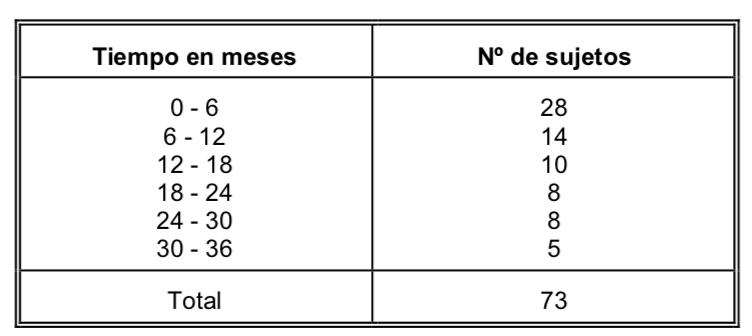
\includegraphics[width=10.44in]{img/1_1}

\textbf{a)} Calcule las frecuencias relativas y porcentajes de los distintos intervalos.

\textbf{b)} Calcule los puntos medios de los intervalos.

\textbf{c)} Calcule las frecuencias absolutas y porcentajes acumulados

\textbf{d)} Construya el histograma, polígono de frecuencias y polígono acumulativo

\hypertarget{soluciuxf3n-13}{%
\subsection{Solución}\label{soluciuxf3n-13}}

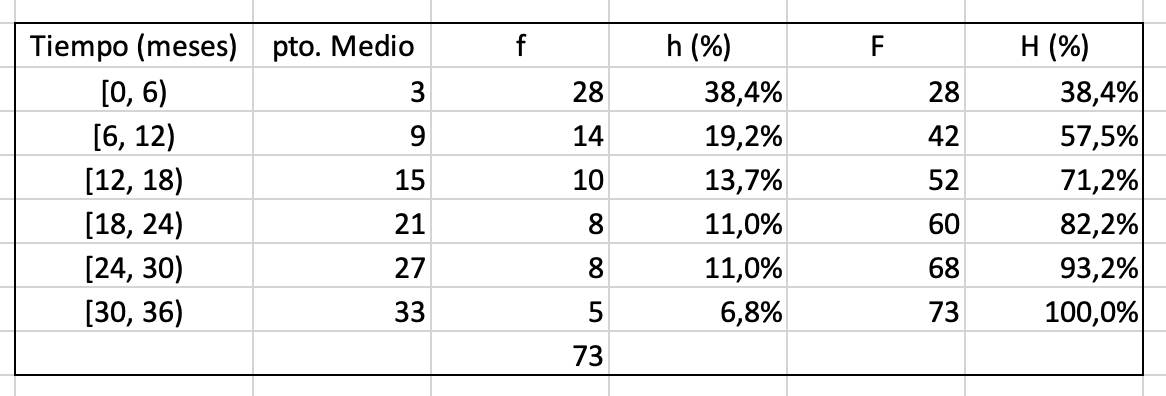
\includegraphics[width=16.19in]{img/1_2}

Tabla construída siguiendo la \href{https://1fjmanzano.github.io/bioestadistica/tablas-de-frecuencias.html\#tabla-de-frecuencias-pr\%C3\%A1ctica-con-excel}{Práctica con Excel© del Curso de Bioestadística}

\hypertarget{pregunta-test-10}{%
\section{Pregunta test}\label{pregunta-test-10}}

Elija la afirmación correcta:

\begin{enumerate}
\def\labelenumi{\alph{enumi})}
\tightlist
\item
  Los valores de cualquier variable deben ser agrupados en intervalos.
\item
  Las variables deben ofrecer valores que no se repitan en los diferentes individuos.
\item
  Las modalidades de una variable deben poder ser observadas en todos los individuos.
\item
  Los individuos pueden poseer diferentes modalidades de la misma variable.
\item
  Todo lo anterior es falso.
\end{enumerate}

\hypertarget{soluciuxf3n-14}{%
\subsection{Solución}\label{soluciuxf3n-14}}

\begin{enumerate}
\def\labelenumi{\alph{enumi})}
\setcounter{enumi}{2}
\tightlist
\item
  \href{https://1fjmanzano.github.io/bioestadistica/tipos-de-variables.html}{Explicación}
\end{enumerate}

\hypertarget{pregunta-test-11}{%
\section{Pregunta test}\label{pregunta-test-11}}

Elija la opción correcta.

\begin{enumerate}
\def\labelenumi{\alph{enumi})}
\tightlist
\item
  Un parámetro es algo calculado sobre cada individuo.
\item
  Un parámetro es calculado sobre la muestra.
\item
  Una variable se calcula sobre los parámetros de una población.
\item
  Un estadístico se calcula sobre la población.
\item
  Nada de lo anterior es correcto.
\end{enumerate}

\hypertarget{soluciuxf3n-15}{%
\subsection{Solución}\label{soluciuxf3n-15}}

\begin{enumerate}
\def\labelenumi{\alph{enumi})}
\setcounter{enumi}{4}
\tightlist
\item
  \href{https://1fjmanzano.github.io/bioestadistica/conceptos-previos.html}{Explicación}
\end{enumerate}

\hypertarget{pregunta-test-12}{%
\section{Pregunta test}\label{pregunta-test-12}}

Disponemos de la distribución de edades de los individuos de una población. El número de ellos que no es mayor de edad, es:

\begin{enumerate}
\def\labelenumi{\alph{enumi})}
\tightlist
\item
  Una frecuencia relativa.
\item
  Una frecuencia absoluta.
\item
  Una frecuencia acumulada.
\item
  Una variable numérica.
\item
  Una variable cualitativa.
\end{enumerate}

\hypertarget{soluciuxf3n-16}{%
\subsection{Solución}\label{soluciuxf3n-16}}

\begin{enumerate}
\def\labelenumi{\alph{enumi})}
\setcounter{enumi}{2}
\tightlist
\item
  \href{https://1fjmanzano.github.io/bioestadistica/tablas-de-frecuencias.html}{Explicación}
\end{enumerate}

\hypertarget{pregunta-test-13}{%
\section{Pregunta test}\label{pregunta-test-13}}

Conocemos la distribución de estudiantes entre las distintas facultades del campus Viriato. El número de estudiantes de Enfermería es:

\begin{enumerate}
\def\labelenumi{\alph{enumi})}
\tightlist
\item
  Una frecuencia relativa.
\item
  Una frecuencia absoluta.
\item
  Una frecuencia acumulada.
\item
  Un porcentaje.
\item
  Una variable cualitativa.
\end{enumerate}

\hypertarget{soluciuxf3n-17}{%
\subsection{Solución}\label{soluciuxf3n-17}}

\begin{enumerate}
\def\labelenumi{\alph{enumi})}
\setcounter{enumi}{1}
\tightlist
\item
  \href{https://1fjmanzano.github.io/bioestadistica/tablas-de-frecuencias.html}{Explicación}
\end{enumerate}

\hypertarget{pregunta-test-14}{%
\section{Pregunta test}\label{pregunta-test-14}}

Se llama parámetro a:

\begin{enumerate}
\def\labelenumi{\alph{enumi})}
\tightlist
\item
  Una función de valor numérico definida sobre alguna característica observable en los individuos de una población.
\item
  Una función definida sobre los valores numéricos de una muestra.
\item
  Cualquier variable observable de una población
\item
  Las variables numéricas de la muestra
\item
  Cualquier función sobre las variables observadas
\end{enumerate}

\hypertarget{soluciuxf3n-18}{%
\subsection{Solución}\label{soluciuxf3n-18}}

\begin{enumerate}
\def\labelenumi{\alph{enumi})}
\tightlist
\item
  \href{https://1fjmanzano.github.io/bioestadistica/conceptos-previos.html}{Explicación}
\end{enumerate}

\hypertarget{pregunta-test-15}{%
\section{Pregunta test}\label{pregunta-test-15}}

El grado de satisfacción (poco/regular/mucho) con la política española la trataría como:

\begin{enumerate}
\def\labelenumi{\alph{enumi})}
\tightlist
\item
  una variable cualitativa nominal.
\item
  una variable cuantitativa discreta.
\item
  una variable cualitativa ordinal.
\item
  una variable numérica continua.
\item
  ninguna de las anteriores es correcta.
\end{enumerate}

\hypertarget{soluciuxf3n-19}{%
\subsection{Solución}\label{soluciuxf3n-19}}

\begin{enumerate}
\def\labelenumi{\alph{enumi})}
\setcounter{enumi}{2}
\tightlist
\item
  \href{https://1fjmanzano.github.io/bioestadistica/tipos-de-variables.html}{Explicación}
\end{enumerate}

\hypertarget{pregunta-test-16}{%
\section{Pregunta test}\label{pregunta-test-16}}

Con respecto a la modalidades de una variable cualquiera:

\begin{enumerate}
\def\labelenumi{\alph{enumi})}
\tightlist
\item
  Pueden siempre agruparse en clases.
\item
  Deben formar un sistema exhaustivo.
\item
  No pueden agruparse en intervalos.
\item
  No tienen porqué formar un sistema excluyente.
\item
  Solo dos son correctas.
\end{enumerate}

\hypertarget{soluciuxf3n-20}{%
\subsection{Solución}\label{soluciuxf3n-20}}

\begin{enumerate}
\def\labelenumi{\alph{enumi})}
\setcounter{enumi}{1}
\tightlist
\item
  \href{https://1fjmanzano.github.io/bioestadistica/tipos-de-variables.html}{Explicación}
\end{enumerate}

\hypertarget{pregunta-test-17}{%
\section{Pregunta test}\label{pregunta-test-17}}

Cuando hablamos de número de cumpleaños que ha tenido una persona estamos ante:

\begin{enumerate}
\def\labelenumi{\alph{enumi})}
\tightlist
\item
  Una variable cualitativa ordinal.
\item
  Una variable cualitativa nominal.
\item
  Una variable cuantitativa discreta.
\item
  Una variable cuantitativa continua.
\item
  El número de cumpleaños no es una variable.
\end{enumerate}

\hypertarget{soluciuxf3n-21}{%
\subsection{Solución}\label{soluciuxf3n-21}}

\begin{enumerate}
\def\labelenumi{\alph{enumi})}
\setcounter{enumi}{2}
\tightlist
\item
  \href{https://1fjmanzano.github.io/bioestadistica/tipos-de-variables.html}{Explicación}
\end{enumerate}

\hypertarget{pregunta-test-18}{%
\section{Pregunta test}\label{pregunta-test-18}}

Las frecuencias acumuladas tienen sentido para:

\begin{enumerate}
\def\labelenumi{\alph{enumi})}
\tightlist
\item
  Variables ordinales
\item
  Variables numéricas
\item
  Variables nominales
\item
  Todas son correctas.
\item
  Las opciones a) y b) son correctas.
\end{enumerate}

\hypertarget{soluciuxf3n-22}{%
\subsection{Solución}\label{soluciuxf3n-22}}

\begin{enumerate}
\def\labelenumi{\alph{enumi})}
\setcounter{enumi}{4}
\tightlist
\item
  \href{https://1fjmanzano.github.io/bioestadistica/tablas-de-frecuencias.html}{Explicación}
\end{enumerate}

\hypertarget{pregunta-test-19}{%
\section{Pregunta test}\label{pregunta-test-19}}

Disponemos de la distribución de edades de los individuos de una población. El número de ellos que tiene dos o menos hijos es:

\begin{enumerate}
\def\labelenumi{\alph{enumi})}
\tightlist
\item
  Una variable cualitativa.
\item
  Una variable numérica.
\item
  Una frecuencia acumulada.
\item
  Son correctas a) y b)
\item
  Ninguna es correcta.
\end{enumerate}

\hypertarget{soluciuxf3n-23}{%
\subsection{Solución}\label{soluciuxf3n-23}}

\begin{enumerate}
\def\labelenumi{\alph{enumi})}
\setcounter{enumi}{2}
\tightlist
\item
  \href{https://1fjmanzano.github.io/bioestadistica/tablas-de-frecuencias.html}{Explicación}
\end{enumerate}

\hypertarget{pregunta-test-20}{%
\section{Pregunta test}\label{pregunta-test-20}}

Los principales objetivos de la estadística descriptiva son:

\begin{enumerate}
\def\labelenumi{\alph{enumi})}
\tightlist
\item
  Sintetizar la información contenida en los datos.
\item
  Aportar resúmenes significativos de las distribuciones.
\item
  Contribuye a la realización de los posteriores análisis estadísticos.
\item
  Todos son correctos.
\end{enumerate}

\hypertarget{soluciuxf3n-24}{%
\subsection{Solución}\label{soluciuxf3n-24}}

\begin{enumerate}
\def\labelenumi{\alph{enumi})}
\setcounter{enumi}{3}
\tightlist
\item
  \href{https://1fjmanzano.github.io/bioestadistica/an\%C3\%A1lisis-exploratorio-de-datos.html}{Explicación}
\end{enumerate}

\hypertarget{pregunta-test-21}{%
\section{Pregunta test}\label{pregunta-test-21}}

El tipo de variable cualitativa que sus valores o categorías no pueden ser ordenados, se denomina:

\begin{enumerate}
\def\labelenumi{\alph{enumi})}
\tightlist
\item
  Variable ordinal.
\item
  Variable discreta.
\item
  Variable nominal.
\item
  Variable continua.
\end{enumerate}

\hypertarget{soluciuxf3n-25}{%
\subsection{Solución}\label{soluciuxf3n-25}}

\begin{enumerate}
\def\labelenumi{\alph{enumi})}
\setcounter{enumi}{2}
\tightlist
\item
  \href{https://1fjmanzano.github.io/bioestadistica/tipos-de-variables.html}{Explicación}
\end{enumerate}

\hypertarget{pregunta-test-22}{%
\section{Pregunta test}\label{pregunta-test-22}}

¿A qué fase del proceso de investigación pertenece la relación de los objetivos e hipótesis de la investigación?

\begin{enumerate}
\def\labelenumi{\alph{enumi})}
\tightlist
\item
  Fase conceptual.
\item
  Fase Metodológica.
\item
  Fase Empírica.
\item
  Fase de análisis e interpretación de los datos.
\end{enumerate}

\hypertarget{soluciuxf3n-26}{%
\subsection{Solución}\label{soluciuxf3n-26}}

\begin{enumerate}
\def\labelenumi{\alph{enumi})}
\tightlist
\item
  \href{https://www.salusplay.com/apuntes/apuntes-metodologia-de-la-investigacion/tema-4-el-proceso-de-investigacion-fases-de-realizacion-de-una-investigacion-cientifica/2}{Explicación}
\end{enumerate}

\hypertarget{anuxe1lisis-descriptivo-y-gruxe1fico-de-datos-cuantitativos}{%
\chapter{Análisis Descriptivo y Gráfico de datos cuantitativos}\label{anuxe1lisis-descriptivo-y-gruxe1fico-de-datos-cuantitativos}}

En este capítulo se resolverán problemas relativos a:

\begin{itemize}
\tightlist
\item
  Medidas de tendencia central: Media, Moda, Mediana.
\item
  Medidas de dispersión: Recorrido, Varianza, Desviación típica, Coeficiente de variación, Recorrido intercuartílico. Error estándar.
\item
  Representaciones gráficas: Diagrama de barras, Pictogramas, Cartogramas,
\end{itemize}

\hypertarget{pregunta-test-23}{%
\section{Pregunta test}\label{pregunta-test-23}}

Cuál de las siguientes medidas define mejor la tendencia central de los datos: 5 , 4, 42, 4, 6

\begin{enumerate}
\def\labelenumi{\alph{enumi})}
\tightlist
\item
  La mediana.
\item
  La media.
\item
  El sesgo
\item
  El rango.
\item
  La proporción.
\end{enumerate}

\hypertarget{soluciuxf3n-27}{%
\subsection{Solución}\label{soluciuxf3n-27}}

\begin{enumerate}
\def\labelenumi{\alph{enumi})}
\tightlist
\item
  \href{https://1fjmanzano.github.io/bioestadistica/medidas-de-posicio\%CC\%81n-dispersio\%CC\%81n-y-forma.html\#medidas-de-posicio\%CC\%81n-centrales}{Explicación}
\end{enumerate}

\hypertarget{pregunta-test-24}{%
\section{Pregunta test}\label{pregunta-test-24}}

Los diagramas de sectores son muy útiles para comparar:

\begin{enumerate}
\def\labelenumi{\alph{enumi})}
\tightlist
\item
  Dos variables cualitativas en una población.
\item
  Dos variables cuantitativas en una población.
\item
  Una variable cualitativa en dos poblaciones.
\item
  Una variable cuantitativa en dos poblaciones.
\item
  Una variable cuantitativa con otra cualitativa.
\end{enumerate}

\hypertarget{soluciuxf3n-28}{%
\subsection{Solución}\label{soluciuxf3n-28}}

\begin{enumerate}
\def\labelenumi{\alph{enumi})}
\setcounter{enumi}{2}
\tightlist
\item
  \href{https://1fjmanzano.github.io/bioestadistica/diagramas-de-barras-y-sectores.html}{Explicación}
\end{enumerate}

\hypertarget{problema-4}{%
\section{Problema}\label{problema-4}}

El siguiente polígono de frecuencias absolutas acumuladas corresponde a la distribución de frecuencias de la variable \(X\) =``Duración en minutos de una consulta médica especializada''.

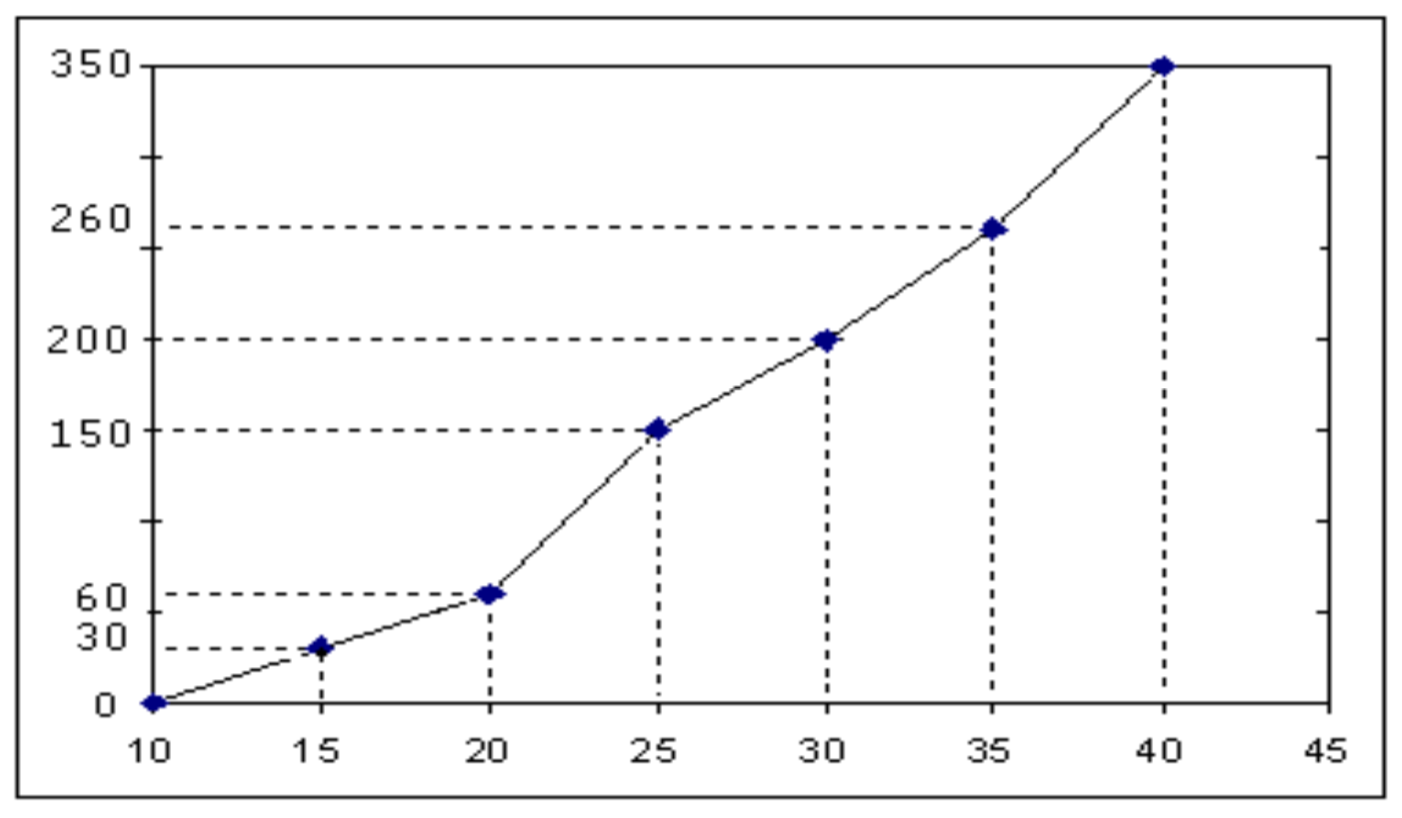
\includegraphics[width=19.47in]{img/2_1}

\textbf{a)} ¿Qué porcentaje de consultas han durado como máximo 30 minutos?

\textbf{b)} ¿Qué porcentaje de consultas han durado entre 25 y 30 minutos?

\hypertarget{soluciuxf3n-29}{%
\subsection{Solución}\label{soluciuxf3n-29}}

Al ser un polígono de frecuencias absolutas acumuladas, vemos que se han contabilizado un total de 350 consultas.

\textbf{a)} Vemos que hay 200 consultas que han durado como máximo 30 minutos. Como \(\frac{200}{350} \approx 0.57\), entonces \textbf{un 57 \% de las consultas han durado entre 25 y 30 minutos}.

\textbf{b)} Entre 25 y 30 minutos, han habido \(200 - 150 = 50\) consultas. Como \(\frac{50}{350} \approx 0.14\), \textbf{un 14 \% de las consultas han durado entre 25 y 30 minutos}

\hypertarget{pregunta-test-25}{%
\section{Pregunta test}\label{pregunta-test-25}}

En cuanto a la presentación ordenada del estudio de una variable aislada:

\begin{enumerate}
\def\labelenumi{\alph{enumi})}
\tightlist
\item
  Lo más informativo es mostrar las medidas de tendencia central.
\item
  Lo más informativo es mostrar las medidas de dispersión.
\item
  Se deben presentar todos los valores observados de la variable, uno a uno, de menor a mayor.
\item
  Las representaciones gráficas dan más información que las tablas de frecuencia.
\item
  A veces no tiene sentido usar frecuencias acumuladas.
\end{enumerate}

\hypertarget{soluciuxf3n-30}{%
\subsection{Solución}\label{soluciuxf3n-30}}

\begin{enumerate}
\def\labelenumi{\alph{enumi})}
\setcounter{enumi}{4}
\tightlist
\item
  \href{https://1fjmanzano.github.io/bioestadistica/otros-gra\%CC\%81ficos.html}{Explicación}
\end{enumerate}

\hypertarget{pregunta-test-26}{%
\section{Pregunta test}\label{pregunta-test-26}}

En las representaciones gráficas de variables cualitativas, la regla fundamental a tener en cuenta es:

\begin{enumerate}
\def\labelenumi{\alph{enumi})}
\tightlist
\item
  Las alturas en cada modalidad son proporcionales al valor de la variable.
\item
  Las áreas para cada modalidad son proporcionales al valor de la variable.
\item
  Las áreas para cada modalidad son proporcionales a las frecuencias acumuladas.
\item
  Las áreas para cada modalidad son proporcionales a las frecuencias absolutas o relativas.
\item
  Las alturas para cada modalidad son proporcionales a las frecuencias acumuladas.
\end{enumerate}

\hypertarget{soluciuxf3n-31}{%
\subsection{Solución}\label{soluciuxf3n-31}}

\begin{enumerate}
\def\labelenumi{\alph{enumi})}
\setcounter{enumi}{3}
\tightlist
\item
  \href{https://1fjmanzano.github.io/bioestadistica/diagramas-de-barras-y-sectores.html}{Explicación}
\end{enumerate}

\hypertarget{pregunta-test-27}{%
\section{Pregunta test}\label{pregunta-test-27}}

Entre las representaciones gráficas para variables cualitativas tenemos:

\begin{enumerate}
\def\labelenumi{\alph{enumi})}
\tightlist
\item
  Histogramas.
\item
  Diagramas integrales.
\item
  Diagramas diferenciales.
\item
  Diagramas de cajas y bigotes.
\item
  Nada de lo anterior.
\end{enumerate}

\hypertarget{soluciuxf3n-32}{%
\subsection{Solución}\label{soluciuxf3n-32}}

\begin{enumerate}
\def\labelenumi{\alph{enumi})}
\setcounter{enumi}{3}
\tightlist
\item
  \href{https://1fjmanzano.github.io/bioestadistica/diagramas-de-barras-y-sectores.html}{Explicación}
\end{enumerate}

\hypertarget{pregunta-test-28}{%
\section{Pregunta test}\label{pregunta-test-28}}

De los siguientes conceptos indique el que no tenga sentido:

\begin{enumerate}
\def\labelenumi{\alph{enumi})}
\tightlist
\item
  Diagrama de barras para la variable ``Grupo sanguíneo''
\item
  Pictograma para la variable ``Altura''
\item
  Diagrama integral para la variable ``Nivel de colesterol''
\item
  Diagrama de sectores para la variable ``Sexo''
\item
  Histograma para la variable ``Peso''
\end{enumerate}

\hypertarget{soluciuxf3n-33}{%
\subsection{Solución}\label{soluciuxf3n-33}}

\begin{enumerate}
\def\labelenumi{\alph{enumi})}
\setcounter{enumi}{1}
\tightlist
\item
  \href{https://1fjmanzano.github.io/bioestadistica/otros-gra\%CC\%81ficos.html}{Explicación}
\end{enumerate}

\hypertarget{pregunta-test-29}{%
\section{Pregunta test}\label{pregunta-test-29}}

Si queremos representar gráficamente los porcentajes de una variable cuantitativa continua debemos usar:

\begin{enumerate}
\def\labelenumi{\alph{enumi})}
\tightlist
\item
  Pictogramas
\item
  Diagrama de barras
\item
  Diagrama diferencial acumulado
\item
  Histograma
\item
  No existe gráfica posible
\end{enumerate}

\hypertarget{soluciuxf3n-34}{%
\subsection{Solución}\label{soluciuxf3n-34}}

\begin{enumerate}
\def\labelenumi{\alph{enumi})}
\setcounter{enumi}{3}
\tightlist
\item
  \href{https://1fjmanzano.github.io/bioestadistica/histogramas.html}{Explicación}
\end{enumerate}

\hypertarget{pregunta-test-30}{%
\section{Pregunta test}\label{pregunta-test-30}}

Los gráficos indicados para variables cualitativas son:

\begin{enumerate}
\def\labelenumi{\alph{enumi})}
\item
  Los diagramas de barras y los histogramas
\item
  Los diagramas de barras, los de sectores y los pictogramas
\item
  Los histogramas y pictogramas
\item
  Sólo los diagramas de barras
\item
  Los diagramas integrales
\item
  \href{https://1fjmanzano.github.io/bioestadistica/diagramas-de-barras-y-sectores.html}{Explicación}
\end{enumerate}

\hypertarget{pregunta-test-31}{%
\section{Pregunta test}\label{pregunta-test-31}}

¿Qué gráfico elegirías para representar una las respuestas a una encuesta sobre el número de hijos que tiene la población?

\begin{enumerate}
\def\labelenumi{\alph{enumi})}
\tightlist
\item
  Histograma
\item
  Diagrama de sectores
\item
  Pictograma
\item
  Diagrama de Barras
\item
  Ninguna de las anteriores
\end{enumerate}

\hypertarget{soluciuxf3n-35}{%
\subsection{Solución}\label{soluciuxf3n-35}}

\begin{enumerate}
\def\labelenumi{\alph{enumi})}
\setcounter{enumi}{3}
\tightlist
\item
  \href{https://1fjmanzano.github.io/bioestadistica/diagramas-de-barras-y-sectores.html}{Explicación}
\end{enumerate}

\hypertarget{pregunta-test-32}{%
\section{Pregunta test}\label{pregunta-test-32}}

Para comparar la variabilidad relativa de la tensión arterial diastólica y el nivel de colesterol en sangre de una serie de individuos, utilizamos

\begin{enumerate}
\def\labelenumi{\alph{enumi})}
\tightlist
\item
  Las desviaciones típicas.
\item
  Los rangos.
\item
  Los coeficientes de variación.
\item
  La diferencia de las medias.
\item
  La diferencia de las varianzas.
\end{enumerate}

\hypertarget{soluciuxf3n-36}{%
\subsection{Solución}\label{soluciuxf3n-36}}

\begin{enumerate}
\def\labelenumi{\alph{enumi})}
\setcounter{enumi}{2}
\tightlist
\item
  \href{https://1fjmanzano.github.io/bioestadistica/medidas-de-posicio\%CC\%81n-dispersio\%CC\%81n-y-forma.html}{Explicación}
\end{enumerate}

\hypertarget{pregunta-test-33}{%
\section{Pregunta test}\label{pregunta-test-33}}

La media aritmética de una variable cuantitativa:

\begin{enumerate}
\def\labelenumi{\alph{enumi})}
\tightlist
\item
  Es siempre un valor de la variable.
\item
  No tiene sentido calcularla para variables discretas.
\item
  Es el valor más representativo de una modalidad.
\item
  Si la variable es discreta, puede no ser única.
\item
  Existe siempre.
\end{enumerate}

\hypertarget{soluciuxf3n-37}{%
\subsection{Solución}\label{soluciuxf3n-37}}

\begin{enumerate}
\def\labelenumi{\alph{enumi})}
\setcounter{enumi}{4}
\tightlist
\item
  \href{https://1fjmanzano.github.io/bioestadistica/medidas-de-posicio\%CC\%81n-dispersio\%CC\%81n-y-forma.html\#medidas-de-posicio\%CC\%81n-centrales}{Explicación}
\end{enumerate}

\hypertarget{pregunta-test-34}{%
\section{Pregunta test}\label{pregunta-test-34}}

Las siguientes medidas son todas de centralización, excepto:

\begin{enumerate}
\def\labelenumi{\alph{enumi})}
\tightlist
\item
  La media.
\item
  La moda.
\item
  La mediana.
\item
  Rango intercuartílico.
\item
  El percentil 50.
\end{enumerate}

\hypertarget{soluciuxf3n-38}{%
\subsection{Solución}\label{soluciuxf3n-38}}

\begin{enumerate}
\def\labelenumi{\alph{enumi})}
\setcounter{enumi}{3}
\tightlist
\item
  \href{https://1fjmanzano.github.io/bioestadistica/medidas-de-posicio\%CC\%81n-dispersio\%CC\%81n-y-forma.html\#medidas-de-posicio\%CC\%81n-centrales}{Explicación}
\end{enumerate}

\hypertarget{pregunta-test-35}{%
\section{Pregunta test}\label{pregunta-test-35}}

En un estudio descriptivo se obtiene una que el peso tiene una media de 60 kg y una desviación típica de 20 kg., mientras que la media de las edades es 15 años, con una desviación típica de 5 años. Entonces:

\begin{enumerate}
\def\labelenumi{\alph{enumi})}
\tightlist
\item
  Hay más dispersión en pesos que en edades.
\item
  Hay más dispersión en edades que en pesos.
\item
  Peso y edad están dispersos de modo equivalente.
\item
  No tiene sentido compararlos al no coincidir las unidades de medida.
\item
  Para comparar ambas dispersiones debemos usar la covarianza.
\end{enumerate}

\hypertarget{soluciuxf3n-39}{%
\subsection{Solución}\label{soluciuxf3n-39}}

\begin{enumerate}
\def\labelenumi{\alph{enumi})}
\setcounter{enumi}{2}
\tightlist
\item
  \href{https://1fjmanzano.github.io/bioestadistica/medidas-de-posicio\%CC\%81n-dispersio\%CC\%81n-y-forma.html}{Explicación}
\end{enumerate}

\hypertarget{pregunta-test-36}{%
\section{Pregunta test}\label{pregunta-test-36}}

¿Cuál de las siguientes características no se corresponde con el concepto de mediana?

\begin{enumerate}
\def\labelenumi{\alph{enumi})}
\tightlist
\item
  Es el centro de gravedad de la distribución.
\item
  No se ve afectada por los valores extremos.
\item
  Deja por debajo el mismo número de datos que por encima.
\item
  Es el segundo cuartil.
\item
  Todo lo anterior se corresponde con la mediana.
\end{enumerate}

\hypertarget{soluciuxf3n-40}{%
\subsection{Solución}\label{soluciuxf3n-40}}

\begin{enumerate}
\def\labelenumi{\alph{enumi})}
\tightlist
\item
  \href{https://1fjmanzano.github.io/bioestadistica/medidas-de-posicio\%CC\%81n-dispersio\%CC\%81n-y-forma.html\#medidas-de-posicio\%CC\%81n-centrales}{Explicación}
\end{enumerate}

\hypertarget{pregunta-test-37}{%
\section{Pregunta test}\label{pregunta-test-37}}

Señale cuál de las siguientes afirmaciones es falsa:

\begin{enumerate}
\def\labelenumi{\alph{enumi})}
\tightlist
\item
  La media aritmética es siempre el centro de gravedad de la distribución.
\item
  En una distribución continua simétrica, media y mediana coinciden.
\item
  La media aritmética cambia cuando cambia algún dato.
\item
  La mediana no siempre cambia cuando lo hace algún dato.
\item
  En las distribuciones continuas simétricas todas las medidas de centralización coinciden.
\end{enumerate}

\hypertarget{soluciuxf3n-41}{%
\subsection{Solución}\label{soluciuxf3n-41}}

\begin{enumerate}
\def\labelenumi{\alph{enumi})}
\setcounter{enumi}{4}
\tightlist
\item
  \href{https://www.statisticshowto.com/what-is-a-bimodal-distribution/}{Explicación}
\end{enumerate}

\hypertarget{pregunta-test-38}{%
\section{Pregunta test}\label{pregunta-test-38}}

El coeficiente de variación:

\begin{enumerate}
\def\labelenumi{\alph{enumi})}
\tightlist
\item
  Permite comparar la dispersión de dos poblaciones.
\item
  Es menor que la media.
\item
  Es menor que la desviación típica.
\item
  No depende de la media ni la desviación típica.
\item
  Depende de la escala que se use al medir la variable.
\end{enumerate}

\hypertarget{soluciuxf3n-42}{%
\subsection{Solución}\label{soluciuxf3n-42}}

\begin{enumerate}
\def\labelenumi{\alph{enumi})}
\tightlist
\item
  \href{https://en.wikipedia.org/wiki/Coefficient_of_variation}{Explicación}
\end{enumerate}

\hypertarget{pregunta-test-39}{%
\section{Pregunta test}\label{pregunta-test-39}}

Se pide a unos enfermos que valoren su grado de mejoría tras un tratamiento en una escala de 1 a 5. De la siguiente colección de posibilidades, cuál cree que resume mejor los mismos:

\begin{enumerate}
\def\labelenumi{\alph{enumi})}
\tightlist
\item
  Media, Mediana y Moda.
\item
  Percentil 25, Percentil 50, Percentil 75.
\item
  Media y desviación típica.
\item
  Mediana y desviación típica.
\item
  Rango
\end{enumerate}

\hypertarget{soluciuxf3n-43}{%
\subsection{Solución}\label{soluciuxf3n-43}}

\begin{enumerate}
\def\labelenumi{\alph{enumi})}
\setcounter{enumi}{1}
\tightlist
\item
  \href{https://1fjmanzano.github.io/bioestadistica/medidas-de-posicio\%CC\%81n-dispersio\%CC\%81n-y-forma.html\#medidas-de-dispersio\%CC\%81n}{Explicación}
\end{enumerate}

\hypertarget{pregunta-test-40}{%
\section{Pregunta test}\label{pregunta-test-40}}

De las siguientes medidas, cuáles podria utilizar para argumentar en favor o en contra de la asimetría de la variable edad:

\begin{enumerate}
\def\labelenumi{\alph{enumi})}
\tightlist
\item
  Percentil 25 y percentil 75.
\item
  Media y Percentil 60.
\item
  Media y mediana
\item
  Media y desviación típica.
\item
  Ninguna de las anteriores.
\end{enumerate}

\hypertarget{soluciuxf3n-44}{%
\subsection{Solución}\label{soluciuxf3n-44}}

\begin{enumerate}
\def\labelenumi{\alph{enumi})}
\setcounter{enumi}{2}
\tightlist
\item
  \href{https://1fjmanzano.github.io/bioestadistica/medidas-de-forma.html}{Explicación}
\end{enumerate}

\hypertarget{pregunta-test-41}{%
\section{Pregunta test}\label{pregunta-test-41}}

La pregunta: ¿qué nivel de colesterol sólo es superado por el 5\% de los individuos?, tiene por respuesta:

\begin{enumerate}
\def\labelenumi{\alph{enumi})}
\tightlist
\item
  El percentil 95.
\item
  El percentil 5.
\item
  Los percentiles 2,5 y 97,5
\item
  95\%.
\item
  Nada de lo anterior.
\end{enumerate}

\hypertarget{soluciuxf3n-45}{%
\subsection{Solución}\label{soluciuxf3n-45}}

\begin{enumerate}
\def\labelenumi{\alph{enumi})}
\tightlist
\item
  \href{https://1fjmanzano.github.io/bioestadistica/medidas-de-posicio\%CC\%81n-dispersio\%CC\%81n-y-forma.html\#medidas-de-posicio\%CC\%81n-no-centrales}{Explicación}
\end{enumerate}

\hypertarget{pregunta-test-42}{%
\section{Pregunta test}\label{pregunta-test-42}}

Qué peso no llega a alcanzar el 40\% de los individuos de una población:

\begin{enumerate}
\def\labelenumi{\alph{enumi})}
\tightlist
\item
  El 40\%.
\item
  El 60\%.
\item
  El percentil 60.
\item
  El percentil 40.
\item
  Los percentiles 20 y 60.
\end{enumerate}

\hypertarget{soluciuxf3n-46}{%
\subsection{Solución}\label{soluciuxf3n-46}}

\begin{enumerate}
\def\labelenumi{\alph{enumi})}
\setcounter{enumi}{3}
\tightlist
\item
  \href{https://1fjmanzano.github.io/bioestadistica/medidas-de-posicio\%CC\%81n-dispersio\%CC\%81n-y-forma.html\#medidas-de-posicio\%CC\%81n-no-centrales}{Explicación}
\end{enumerate}

\hypertarget{pregunta-test-43}{%
\section{Pregunta test}\label{pregunta-test-43}}

La media aritmética de una variable discreta:

\begin{enumerate}
\def\labelenumi{\alph{enumi})}
\tightlist
\item
  Puede ser un valor de la variable.
\item
  No debería ser utilizada como medida de centralización.
\item
  Es lo mismo que el percentil 50.
\item
  Puede no ser única.
\item
  Todo lo anterior es falso.
\end{enumerate}

\hypertarget{soluciuxf3n-47}{%
\subsection{Solución}\label{soluciuxf3n-47}}

\begin{enumerate}
\def\labelenumi{\alph{enumi})}
\tightlist
\item
  \href{https://1fjmanzano.github.io/bioestadistica/medidas-de-posicio\%CC\%81n-dispersio\%CC\%81n-y-forma.html\#medidas-de-posicio\%CC\%81n-centrales}{Explicación}
\end{enumerate}

\hypertarget{pregunta-test-44}{%
\section{Pregunta test}\label{pregunta-test-44}}

Se pregunta a los individuos su opinión sobre una cuestión, pudiendo valorar estos su respuesta en términos de: en contra, en parte a favor, muy a favor, totalmente de acuerdo. Elija la afirmación correcta:

\begin{enumerate}
\def\labelenumi{\alph{enumi})}
\tightlist
\item
  Podemos calcular la media.
\item
  Podemos calcular el coeficiente de variación.
\item
  La variable es de tipo ordinal
\item
  La variable es de tipo cualitativo nominal.
\item
  Nada de lo anterior es cierto.
\end{enumerate}

\hypertarget{soluciuxf3n-48}{%
\subsection{Solución}\label{soluciuxf3n-48}}

\begin{enumerate}
\def\labelenumi{\alph{enumi})}
\setcounter{enumi}{2}
\tightlist
\item
  \href{https://1fjmanzano.github.io/bioestadistica/tipos-de-variables.html}{Explicación}
\end{enumerate}

\hypertarget{pregunta-test-45}{%
\section{Pregunta test}\label{pregunta-test-45}}

En una población, el 70\% de las alturas consideradas ``más normales'' se encuentran:

\begin{enumerate}
\def\labelenumi{\alph{enumi})}
\tightlist
\item
  Por encima del percentil 70.
\item
  Por debajo del cuantil 0,30
\item
  Entre el percentil 30 y el 70
\item
  Entre el percentil 15 y el 85.
\item
  Entre la media y la mediana.
\end{enumerate}

\hypertarget{soluciuxf3n-49}{%
\subsection{Solución}\label{soluciuxf3n-49}}

\begin{enumerate}
\def\labelenumi{\alph{enumi})}
\setcounter{enumi}{3}
\tightlist
\item
  \href{https://1fjmanzano.github.io/bioestadistica/distribuciones-de-probabilidad.html\#distribucio\%CC\%81n-normal}{Explicación}
\end{enumerate}

\hypertarget{pregunta-test-46}{%
\section{Pregunta test}\label{pregunta-test-46}}

Las medidas de centralización, en cuanto a la información que ofrecen sobre una variable numérica, preferimos (por orden, de peor a mejor):

\begin{enumerate}
\def\labelenumi{\alph{enumi})}
\tightlist
\item
  media, mediana, moda
\item
  moda, media, mediana
\item
  media, moda, mediana.
\item
  No se puede en general recomendar una como mejor que las otras.
\item
  Todo lo anterior es falso.
\end{enumerate}

\hypertarget{soluciuxf3n-50}{%
\subsection{Solución}\label{soluciuxf3n-50}}

\begin{enumerate}
\def\labelenumi{\alph{enumi})}
\setcounter{enumi}{3}
\tightlist
\item
  \href{https://1fjmanzano.github.io/bioestadistica/medidas-de-posicio\%CC\%81n-dispersio\%CC\%81n-y-forma.html\#medidas-de-posicio\%CC\%81n-centrales}{Explicación}
\end{enumerate}

\hypertarget{pregunta-test-47}{%
\section{Pregunta test}\label{pregunta-test-47}}

Si una muestra posee valores anómalos, de las siguientes cuál usarías como medida de dispersión:

\begin{enumerate}
\def\labelenumi{\alph{enumi})}
\tightlist
\item
  Varianza.
\item
  Desviación típica.
\item
  Rango intercuartílico.
\item
  Rango.
\item
  Máximo y coeficiente de variación.
\end{enumerate}

\hypertarget{soluciuxf3n-51}{%
\subsection{Solución}\label{soluciuxf3n-51}}

\begin{enumerate}
\def\labelenumi{\alph{enumi})}
\setcounter{enumi}{2}
\tightlist
\item
  \href{https://1fjmanzano.github.io/bioestadistica/medidas-de-posicio\%CC\%81n-dispersio\%CC\%81n-y-forma.html\#medidas-de-dispersio\%CC\%81n}{Explicación}
\end{enumerate}

\hypertarget{pregunta-test-48}{%
\section{Pregunta test}\label{pregunta-test-48}}

Si queremos saber cómo de disperso está una variable relativamente con respecto a la magnitud de los valores centrales de la misma, usaremos:

\begin{enumerate}
\def\labelenumi{\alph{enumi})}
\tightlist
\item
  Varianza.
\item
  Desviación típica.
\item
  Rango intercuartílico.
\item
  Rango.
\item
  Coeficiente de variación.
\end{enumerate}

\hypertarget{soluciuxf3n-52}{%
\subsection{Solución}\label{soluciuxf3n-52}}

\begin{enumerate}
\def\labelenumi{\alph{enumi})}
\setcounter{enumi}{4}
\tightlist
\item
  \href{https://en.wikipedia.org/wiki/Coefficient_of_variation}{Explicación}
\end{enumerate}

\hypertarget{pregunta-test-49}{%
\section{Pregunta test}\label{pregunta-test-49}}

Si el coeficiente de asimetría en una población presenta el valor 0,99 entonces:

\begin{enumerate}
\def\labelenumi{\alph{enumi})}
\tightlist
\item
  La distribución presenta una cola a la derecha.
\item
  La distribución presenta una cola a la izquierda.
\item
  La distribución es más apuntada que la normal.
\item
  La distribución es menos apuntada que la normal.
\item
  La distribución es prácticamente simétrica.
\end{enumerate}

\hypertarget{soluciuxf3n-53}{%
\subsection{Solución}\label{soluciuxf3n-53}}

\begin{enumerate}
\def\labelenumi{\alph{enumi})}
\tightlist
\item
  \href{https://1fjmanzano.github.io/bioestadistica/medidas-de-forma.html}{Explicación}
\end{enumerate}

\hypertarget{pregunta-test-50}{%
\section{Pregunta test}\label{pregunta-test-50}}

Si la media del peso en una población es 60 kg. y la mediana 65kg., entonces afirmamos que la distribución del peso en la población es:

\begin{enumerate}
\def\labelenumi{\alph{enumi})}
\tightlist
\item
  Platicúrtica.
\item
  Mesocúrtica.
\item
  Leptocúrtica.
\item
  Asimétrica.
\item
  Unimodal.
\end{enumerate}

\hypertarget{soluciuxf3n-54}{%
\subsection{Solución}\label{soluciuxf3n-54}}

\begin{enumerate}
\def\labelenumi{\alph{enumi})}
\setcounter{enumi}{3}
\tightlist
\item
  \href{https://1fjmanzano.github.io/bioestadistica/medidas-de-forma.html}{Explicación}
\end{enumerate}

\hypertarget{pregunta-test-51}{%
\section{Pregunta test}\label{pregunta-test-51}}

Si el coeficiente de asimetría en una población presenta el valor -5,22 entonces:

\begin{enumerate}
\def\labelenumi{\alph{enumi})}
\tightlist
\item
  La distribución presenta una cola a la derecha.
\item
  La distribución presenta una cola a la izquierda.
\item
  La distribución es más apuntada que la normal.
\item
  La distribución es menos apuntada que la normal.
\item
  Ese valor de asimetría es imposible.
\end{enumerate}

\hypertarget{soluciuxf3n-55}{%
\subsection{Solución}\label{soluciuxf3n-55}}

\begin{enumerate}
\def\labelenumi{\alph{enumi})}
\setcounter{enumi}{1}
\tightlist
\item
  \href{https://1fjmanzano.github.io/bioestadistica/medidas-de-forma.html}{Explicación}
\end{enumerate}

\hypertarget{pregunta-test-52}{%
\section{Pregunta test}\label{pregunta-test-52}}

Medimos el número de glóbulos rojos y el de blancos en cada individuo de una población. Se observa determinada variabilidad en esas cantidades. Queremos saber de qué tipo de célula se presenta mayor variabilidad

\begin{enumerate}
\def\labelenumi{\alph{enumi})}
\tightlist
\item
  Compararemos las desviaciones típicas.
\item
  Compararemos los rangos.
\item
  Estudiaremos la covarianza.
\item
  Estudiaremos el coeficiente de correlación lineal de Pearson.
\item
  Compararemos los coeficientes de variación.
\end{enumerate}

\hypertarget{soluciuxf3n-56}{%
\subsection{Solución}\label{soluciuxf3n-56}}

\begin{enumerate}
\def\labelenumi{\alph{enumi})}
\setcounter{enumi}{4}
\tightlist
\item
  \href{https://en.wikipedia.org/wiki/Coefficient_of_variation}{Explicación}
\end{enumerate}

\hypertarget{pregunta-test-53}{%
\section{Pregunta test}\label{pregunta-test-53}}

En una muestra de 1000 mujeres se estudia su número de hijos. Si quiero tener el máximo de información sobre la variable del estudio, preferimos:

\begin{enumerate}
\def\labelenumi{\alph{enumi})}
\tightlist
\item
  Media, Mediana y Moda.
\item
  Percentil 25, Percentil 50, Percentil 75.
\item
  Media y desviación típica.
\item
  Media, mediana, cuartiles, asimetría, curtosis y desviación típica.
\item
  Distribución de frecuencias
\end{enumerate}

\hypertarget{soluciuxf3n-57}{%
\subsection{Solución}\label{soluciuxf3n-57}}

\begin{enumerate}
\def\labelenumi{\alph{enumi})}
\setcounter{enumi}{4}
\tightlist
\item
  \href{https://1fjmanzano.github.io/bioestadistica/tablas-de-frecuencias.html}{Explicación}
\end{enumerate}

\hypertarget{pregunta-test-54}{%
\section{Pregunta test}\label{pregunta-test-54}}

El 3\% de los individuos tiene una altura superior a 190cm. El 5\% mide menos de 150cm. Conocemos:

\begin{enumerate}
\def\labelenumi{\alph{enumi})}
\tightlist
\item
  El percentil 3
\item
  El cuantil 0,06
\item
  El percentil 95
\item
  El percentil 97
\item
  Nada de lo anterior.
\end{enumerate}

\hypertarget{soluciuxf3n-58}{%
\subsection{Solución}\label{soluciuxf3n-58}}

\begin{enumerate}
\def\labelenumi{\alph{enumi})}
\setcounter{enumi}{3}
\tightlist
\item
  \href{https://1fjmanzano.github.io/bioestadistica/medidas-de-posicio\%CC\%81n-dispersio\%CC\%81n-y-forma.html\#medidas-de-posicio\%CC\%81n-no-centrales}{Explicación}
\end{enumerate}

\hypertarget{pregunta-test-55}{%
\section{Pregunta test}\label{pregunta-test-55}}

Respecto a las medidas de centralización:

\begin{enumerate}
\def\labelenumi{\alph{enumi})}
\tightlist
\item
  La media no debe usarse en distribuciones muy asimétricas.
\item
  La moda puede no ser única.
\item
  En distribuciones simétricas media, mediana y moda coinciden.
\item
  Las tres anteriores son correctas.
\item
  Sólo la a) y la b) son correctas
\end{enumerate}

\hypertarget{soluciuxf3n-59}{%
\subsection{Solución}\label{soluciuxf3n-59}}

\begin{enumerate}
\def\labelenumi{\alph{enumi})}
\setcounter{enumi}{4}
\tightlist
\item
  \href{https://1fjmanzano.github.io/bioestadistica/medidas-de-forma.html}{Explicación1} y \href{https://www.statisticshowto.com/what-is-a-bimodal-distribution/}{Explicación2}
\end{enumerate}

\hypertarget{pregunta-test-56}{%
\section{Pregunta test}\label{pregunta-test-56}}

El coeficiente de asimetría en una población vale 3. Elija la afirmación correcta:

\begin{enumerate}
\def\labelenumi{\alph{enumi})}
\tightlist
\item
  La distribución presenta una cola a la derecha.
\item
  La distribución presenta una cola a la izquierda.
\item
  La distribución es simétrica.
\item
  La distribución es más apuntada que la normal
\item
  La media es igual a la mediana.
\end{enumerate}

\hypertarget{soluciuxf3n-60}{%
\subsection{Solución}\label{soluciuxf3n-60}}

\begin{enumerate}
\def\labelenumi{\alph{enumi})}
\tightlist
\item
  \href{https://1fjmanzano.github.io/bioestadistica/medidas-de-forma.html}{Explicación}
\end{enumerate}

\hypertarget{pregunta-test-57}{%
\section{Pregunta test}\label{pregunta-test-57}}

¿Cuál de las siguientes medidas define mejor la tendencia central de los datos: 1, 2, 4, 5, 9, 1, 3, 9, 400?

\begin{enumerate}
\def\labelenumi{\alph{enumi})}
\tightlist
\item
  Media.
\item
  Cuantil 0,5.
\item
  Moda
\item
  Desviación típica.
\item
  Ninguna de las anteriores.
\end{enumerate}

\hypertarget{soluciuxf3n-61}{%
\subsection{Solución}\label{soluciuxf3n-61}}

\begin{enumerate}
\def\labelenumi{\alph{enumi})}
\setcounter{enumi}{1}
\tightlist
\item
  \href{https://1fjmanzano.github.io/bioestadistica/medidas-de-posicio\%CC\%81n-dispersio\%CC\%81n-y-forma.html\#medidas-de-posicio\%CC\%81n-no-centrales}{Explicación}
\end{enumerate}

\hypertarget{pregunta-test-58}{%
\section{Pregunta test}\label{pregunta-test-58}}

De las siguientes variables ¿con cuáles NO puedo calcular la media?

\begin{enumerate}
\def\labelenumi{\alph{enumi})}
\tightlist
\item
  temperatura corporal
\item
  pH del estómago
\item
  grupo sanguíneo
\item
  número de glóbulos rojos
\item
  edad
\end{enumerate}

\hypertarget{soluciuxf3n-62}{%
\subsection{Solución}\label{soluciuxf3n-62}}

\begin{enumerate}
\def\labelenumi{\alph{enumi})}
\setcounter{enumi}{2}
\tightlist
\item
  \href{https://1fjmanzano.github.io/bioestadistica/tipos-de-variables.html}{Explicación}
\end{enumerate}

\hypertarget{pregunta-test-59}{%
\section{Pregunta test}\label{pregunta-test-59}}

De las siguientes variables con cuál sería menos adecuado un diagrama de barras?

\begin{enumerate}
\def\labelenumi{\alph{enumi})}
\tightlist
\item
  Número de hijos
\item
  Número de coches que posee la familia
\item
  Número de cigarros fumados al día
\item
  Número de glóbulos rojos
\item
  Número de mascotas.
\end{enumerate}

\hypertarget{soluciuxf3n-63}{%
\subsection{Solución}\label{soluciuxf3n-63}}

\begin{enumerate}
\def\labelenumi{\alph{enumi})}
\setcounter{enumi}{3}
\tightlist
\item
  \href{https://1fjmanzano.github.io/bioestadistica/representaciones-gra\%CC\%81ficas.html}{Explicación}
\end{enumerate}

\hypertarget{pregunta-test-60}{%
\section{Pregunta test}\label{pregunta-test-60}}

Cuál es la mediana de los siguientes datos 22, 5, 9, 11, 10, 14, 7

\begin{enumerate}
\def\labelenumi{\alph{enumi})}
\tightlist
\item
  5
\item
  9
\item
  11
\item
  10
\item
  14
\end{enumerate}

\hypertarget{soluciuxf3n-64}{%
\subsection{Solución}\label{soluciuxf3n-64}}

\begin{enumerate}
\def\labelenumi{\alph{enumi})}
\setcounter{enumi}{3}
\tightlist
\item
  \href{https://1fjmanzano.github.io/bioestadistica/medidas-de-posicio\%CC\%81n-dispersio\%CC\%81n-y-forma.html\#medidas-de-posicio\%CC\%81n-centrales}{Explicación}
\end{enumerate}

\hypertarget{pregunta-test-61}{%
\section{Pregunta test}\label{pregunta-test-61}}

Si el cuantil 0,9 del peso es 70 kilogramos, quiere decir esto:

\begin{enumerate}
\def\labelenumi{\alph{enumi})}
\tightlist
\item
  Que una frecuencia del 70\% individuos pesa más de 70 kilogramos.
\item
  Que una frecuencia del 90\% de individuos pesa más de 70 kilogramos.
\item
  Que una frecuencia del 90\% individuos pesa menos de 70 kilogramos.
\item
  Que una frecuencia de 70\% de individuos pesa menos de 90 kilogramos.
\item
  Todas son falsas.
\end{enumerate}

\hypertarget{soluciuxf3n-65}{%
\subsection{Solución}\label{soluciuxf3n-65}}

\begin{enumerate}
\def\labelenumi{\alph{enumi})}
\setcounter{enumi}{2}
\tightlist
\item
  \href{https://1fjmanzano.github.io/bioestadistica/medidas-de-posicio\%CC\%81n-dispersio\%CC\%81n-y-forma.html\#medidas-de-posicio\%CC\%81n-centrales}{Explicación}
\end{enumerate}

\hypertarget{pregunta-test-62}{%
\section{Pregunta test}\label{pregunta-test-62}}

En una distribución: \(P_{25} = 40\), \(P_{50} =60\) y \(P_{75} =70\).

\begin{enumerate}
\def\labelenumi{\alph{enumi})}
\tightlist
\item
  La distribución es simétrica
\item
  La distribución sugiere asimetría negativa
\item
  La distribución sugiere asimetría positiva
\item
  La distribución es leptocúrtica
\item
  Las opciones a) y d) son ciertas
\end{enumerate}

\hypertarget{soluciuxf3n-66}{%
\subsection{Solución}\label{soluciuxf3n-66}}

\begin{enumerate}
\def\labelenumi{\alph{enumi})}
\setcounter{enumi}{1}
\tightlist
\item
  \href{https://1fjmanzano.github.io/bioestadistica/medidas-de-forma.html}{Explicación}
\end{enumerate}

\hypertarget{pregunta-test-63}{%
\section{Pregunta test}\label{pregunta-test-63}}

En una distribución la mediana es 20 y la media es 26:

\begin{enumerate}
\def\labelenumi{\alph{enumi})}
\tightlist
\item
  Con seguridad hay asimetría negativa
\item
  Con seguridad hay asimetría positiva
\item
  Hay colas hacia la derecha y hacia la izquierda.
\item
  Los datos son simétricos.
\item
  Los datos sugieren una cola hacia la derecha. Habría que estudiarlo con más detalle
\end{enumerate}

\hypertarget{soluciuxf3n-67}{%
\subsection{Solución}\label{soluciuxf3n-67}}

\begin{enumerate}
\def\labelenumi{\alph{enumi})}
\setcounter{enumi}{4}
\tightlist
\item
  \href{https://1fjmanzano.github.io/bioestadistica/medidas-de-forma.html}{Explicación}
\end{enumerate}

\hypertarget{pregunta-test-64}{%
\section{Pregunta test}\label{pregunta-test-64}}

El Rango Intercuartílico:

\begin{enumerate}
\def\labelenumi{\alph{enumi})}
\tightlist
\item
  Es sensible a los datos extremos.
\item
  Es la distancia ente el primer y segundo cuartil.
\item
  Es la raíz cuadrada de la varianza
\item
  Sus unidades son el cuadrado de las variables.
\item
  Mide el grado de dispersión de los datos, independientemente de su causa.
\end{enumerate}

\hypertarget{soluciuxf3n-68}{%
\subsection{Solución}\label{soluciuxf3n-68}}

\begin{enumerate}
\def\labelenumi{\alph{enumi})}
\setcounter{enumi}{4}
\tightlist
\item
  \href{https://1fjmanzano.github.io/bioestadistica/medidas-de-posicio\%CC\%81n-dispersio\%CC\%81n-y-forma.html\#medidas-de-dispersio\%CC\%81n}{Explicación}
\end{enumerate}

\hypertarget{anuxe1lisis-inferencial.-aplicaciones.}{%
\chapter{Análisis Inferencial. Aplicaciones.}\label{anuxe1lisis-inferencial.-aplicaciones.}}

En este capítulo se resolverán problemas relativos a:

\begin{itemize}
\tightlist
\item
  Objetivos del estudio, hipótesis de trabajo e hipótesis estadísticas
\item
  Importancia de las distribuciones de probabilidad en el trabajo práctico
\item
  Estimación puntual y por intervalo
\item
  Verificación de las hipótesis de trabajo: contraste de hipótesis
\end{itemize}

\hypertarget{regresiuxf3n-y-correlaciuxf3n.}{%
\chapter{Regresión y correlación.}\label{regresiuxf3n-y-correlaciuxf3n.}}

En este capítulo se resolverán problemas relativos a:

\begin{itemize}
\tightlist
\item
  Introducción a la regresión y correlación
\item
  Estudio de la representatividad de la recta de regresión
\item
  Otros modelos de regresión
\item
  Correlación
\end{itemize}

\hypertarget{tablas-de-contingencia.}{%
\chapter{Tablas de contingencia.}\label{tablas-de-contingencia.}}

En este capítulo se resolverán problemas relativos a:

\begin{itemize}
\tightlist
\item
  Contrastes de asociación y homogeneidad en tablas bifactoriales
\item
  Coeficientes de asociación
\end{itemize}

\hypertarget{medidas-de-importancia-cluxednica.}{%
\chapter{Medidas de importancia clínica.}\label{medidas-de-importancia-cluxednica.}}

En este capítulo se resolverán problemas relativos a:

\begin{itemize}
\tightlist
\item
  Diferencias entre Proporción, Tasa, Razón, odds.
\item
  Medidas de asociación en tablas 2x2. Riesgo Relativo. Riesgo Absolutos. Odds-Ratio.
\item
  Indicadores estadísticos básicos para evaluar el desempeño de un procedimiento diagnóstico: Sensibilidad y Especificidad. Probabilidades pre y post prueba.
\end{itemize}

  \bibliography{book.bib,packages.bib}

\end{document}
